\section{Experiments}
\label{sec:experiments}
In this section, we conduct experiments to evaluate the effectiveness of TRacer on a large-scale real-world dataset. Besides, we conduct case studies with network visualization techniques.

\subsection{Experimental Setups}
% 主要包括参数设置、数据集描述、指标、对比算法

\subsubsection{Dataset}
We contribute a benchmark dataset including 20 transaction tracing cases in the recent 5 years across three account-based blockchains, i.e., Ethereum, Binance Smart Chain, and Polygon. 
These cases are initialized by various illegal activities containing hacker attacks, Rug-pull, and scams which have caused billions of dollars in losses. 
All these cases are reported by blockchain security companies and verified by experts coming from Certik \footnote{https://www.certik.com/}, Peckchield \footnote{https://peckshield.com/}, Chainalysis \footnote{https://www.chainalysis.com/} and so on.
Some statistics of this dataset are shown in Table \ref{tab:dataset}. 
Note that the transaction data in the dataset is obtained from the open APIs\footnote{https://blockscan.com}.
As we can see, the activities of these cases have acrossed millions of blocks, and we have to trace the money flows of the sources among more than 4 billion transactions.

\begin{table}[t]
  \caption{Statistics of the transaction record data related to the cases }
  \label{tab:dataset}
  \begin{tabular}{l|l|l}
    \hline
    \textbf{Field} & \textbf{Description} & \textbf{Number} \\
    \hline
    Source nodes & \tabincell{l}{The source node related to this\\case, such as the hacker account\\ and the scam contract.} & 20 \\ \hline
    Target nodes & \tabincell{l}{A set of target nodes related to\\this case, such as exchange\\wallets and mixing services.}  & 0.87K \\ \hline
    Blocks & \tabincell{l}{The blocks related to these cases.}  & 23.5M \\ \hline
    Transactions & \tabincell{l}{The transactions contained in the\\blocks related to these cases.} & 4.83B \\ \hline
  \end{tabular}
\end{table}
% Experiments are started from the source node in these cases in order to find the target nodes.

% \begin{table}[t]
%     \caption{Statistics of Cases}
%     \centering
%     \begin{threeparttable}
%         \begin{tabular}{cccccc}
%             \hline
%             Case & Source\tnote{1} & \#Target & \#Node & \#Edge & Block\tnote{2}\\
%             \hline
%             PlusToken & 0xf4a2e & 17 & 68 & 164 & 7993213\\
%             TokenStore & 0x068ac & 5 & 80 & 194 & 7802134\\
%             Cryptopia & 0xd4e79 & 4 & 9 & 24 & 9128188\\
%             Kucoin & 0xeb319 & - & - & - & 10933499\\
%             Upbit & 0xa0987 & - & - & - & 9007863\\
%             \hline
%         \end{tabular}
%         \begin{tablenotes}    
%             \footnotesize              
%             \item[1] Here provides the address prefix of the source node.
%             \item[2] Here provides the block number of the first transaction related to the cases.
%         \end{tablenotes}  
%     \end{threeparttable}
%     \label{tab:cases}
% \end{table}

% \begin{table*}[htb]
%     \caption{Experimental Results.}
%     \centering
%     \begin{threeparttable}
%         \begin{tabular}{cccccccccccccccc}
%             \hline
%              & \multicolumn{3}{c}{PlusToken} & \multicolumn{3}{c}{TokenStore} & \multicolumn{3}{c}{Cryptopia} & \multicolumn{3}{c}{Kucoin} & \multicolumn{3}{c}{Upbit} \\ \cmidrule(r){2-4} \cmidrule(r){5-7} \cmidrule(r){8-10} \cmidrule(r){11-13} \cmidrule(r){14-16}
%             Methods & $D_l$ & $K$ & $R$ & $D_l$ & $K$ & $R$ & $D_l$ & $K$ & $R$ & $D_l$ & $K$ & $P_l$ & $D_l$ & $K$ & $P_l$\\ \hline
%             BFS & 4.0$\times 10^{-9}$ & 3 & \textbf{0.93} &
%                 1.6$\times 10^{-7}$ & 3 & 0.4 &
%                 3.4$\times 10^{-7}$ & 3 & 1.0 &
%                 1.1$\times 10^{-8}$ & 3 & - &
%                 3.8$\times 10^{-9}$ & 3 & -\\
%             Poison & 6.3$\times 10^{-9}$ & 3 & 0 &
%                 1.6$\times 10^{-7}$ & 3 & 0.4 &
%                 2.3$\times 10^{-6}$ & 3 & 1.0 &
%                 2.3$\times 10^{-8}$ & 3 & - &
%                 6.4$\times 10^{-6}$ & 3 & -\\
%             Haircut & 7.6$\times 10^{-9}$ & \textbf{6} & \textbf{0.93} &
%                 8.1$\times 10^{-8}$ & \textbf{6} & \textbf{1.0} &
%                 7.0$\times 10^{-8}$ & 7 & \textbf{1.0}\tnote{*} &
%                 2.0$\times 10^{-5}$ & 4 & - &
%                 4.0$\times 10^{-7}$ & 5 & -\\
%             APPR & 0 & 0 & 0 &
%                 8.1$\times 10^{-4}$ & 5 & 0.4 &
%                 3.1$\times 10^{-4}$ & 7 & \textbf{1.0}\tnote{*} &
%                 6.0$\times 10^{-4}$ & 4 & 0.25 &
%                 2.4$\times 10^{-4}$ & 4 & 0.26\\
%             \hline
%             TTR-base & 4.9$\times 10^{-5}$ & 5 & \textbf{0.93} & 
%                 \textbf{2.0}\bm{$\times$}\textbf{10}$^{-3}$ & 5 & 0.4 & 
%                 4.0$\times 10^{-4}$ & 6 & \textbf{1.0}\tnote{*} & 
%                 \textbf{6.2}\bm{$\times$}\textbf{10}$^{-4}$ & 4 & 0.26 & 
%                 2.8$\times 10^{-4}$ & 6 & 0.44\\
%             TTR-weight & 2.2$\times 10^{-5}$ & \textbf{6} & \textbf{0.93} & 
%                 2.8$\times 10^{-4}$ & \textbf{6} & \textbf{1.0} & 
%                 6.9$\times 10^{-4}$ & 7 & \textbf{1.0}\tnote{*} & 
%                 2.7$\times 10^{-4}$ & 5 & 0.39 & 
%                 4.0$\times 10^{-4}$ & \textbf{8} & \textbf{0.75}\\
%             TTR-time & \textbf{1.2}\bm{$\times$}\textbf{10}$^{-4}$ & 5 & \textbf{0.93} &
%                 1.6$\times 10^{-4}$ & \textbf{6} & \textbf{1.0} &
%                 \textbf{9.6}\bm$\times$\textbf{10}$^{-4}$ & \textbf{10} & \textbf{1.0}\tnote{*} &
%                 2.2$\times 10^{-4}$ & \textbf{7} & \textbf{0.52} & 
%                 \textbf{4.3}\bm$\times$\textbf{10}$^{-4}$ & \textbf{8} & 0.65\\
%              \hline
%         \end{tabular}
%         \begin{tablenotes}    
%             \footnotesize              
%             \item[*] These methods can find some extra suspicious target nodes, referring to Section \ref{sec:case_study_Cryptopia}.
%         \end{tablenotes}
%     \end{threeparttable}
%     \label{tab:experimentations}
% \end{table*}

\subsubsection{Compared Methods}
We compare our method with several baseline blockchain transaction tracing methods. For a fair comparison, we use the general framework of TRacer to reproduce the following comparison methods, including:
\begin{itemize}
    \item \textbf{BFS} \cite{zhao2015graph}: Breadth-First Search, which is the first and the most commonly used transaction tracing method.
    \item \textbf{Poison} \cite{moser2014towards}: A kind of taint analysis technology in blockchain transaction tracing. Each output of a transaction with a dirty input is considered to be tainted in this method.
    \item \textbf{Haircut} \cite{moser2014towards}: A kind of taint analysis technology in blockchain transaction tracing. Each output of a transaction with a dirty input is considered to be tainted partially according to the amount value in this method. 
    \item \textbf{APPR} \cite{andersen2006local}: The approximate personalized PageRank algorithms, which can calculate the relevance of nodes in a network to a given source node with an extremely low cost.
    % \item \textbf{TRacer}: The method we proposed, where the graph construction recognizes the transaction patterns, the TTR and greedy selection are used for graph expansion, and the local community detection is applied in Extract.
    % using a novel local push procedure, and we abbreviate the TTR algorithm with tracing tendency, weight pollution, and temporal reasoning strategies as TTR-base, TTR-weight, and TTR-time respectively.
\end{itemize}

The details of implementing the above transaction tracing technologies can be found in our GitHub page \footnote{https://github.com/wuzhy1ng/BlockchainSpider}.

\subsubsection{Experimental Settings} 
% {\color{blue}Based on the experiences, it is enough for BFS and Poison to trace the 2-order neighbors of the source node, since the increase of order leads to the exponential growth of the size of subgraph in graph expansion for these two methods, bringing great difficulty to transaction auditing.}
%%  !!!! 这段话大有问题
Since the increase of depth can lead to the exponential growth of the size of output graph in BFS and Poison, bringing great difficulty to transaction auditing. During our experiments, we set the upper limit of the tracing depth in these two methods is 2. In addition, we use the Haircut method to trace the ``dirty money'' from the source node until the amount proportion of ``dirty money" of all nodes is less than 0.1\% of that from the source node.
Moreover, we set $\alpha=0.15$, $\epsilon=10^{-3}$ for APPR and TTR, and $\varphi=10^{-3}$, $\beta=0.7$ for TTR to ensure that our method is able to find the paths among the source node and the target nodes with 42-hop at most, according to Proposition \ref{pot:max_depth}.

\subsubsection{Metrics}
we report the average of the following metrics in all cases to measure the effectiveness of transaction tracing:
% We use the following metrics to measure the effectiveness of transaction tracing:
\begin{itemize}
    \item \textbf{Recall}: The recall evaluates how many target nodes can be traced by a method, which is defined as: $Recall = \frac{|V_t|}{|\bar{V_t}|}$, where $|V_t|$ is the number of traced target nodes and $|\bar{V_t}|$ is the number of all target nodes in a case.
    
    \item \textbf{Number of nodes}: This metric measures the number of nodes in the output graph of a case. A smaller output graph with recall ensured is easier for expert auditing.
    % Ensuring the recall, the fewer node number, the more conducive to expert verification.
    
    \item \textbf{Tracing depth}: This metric measures how deep can a transaction tracing method traverse the transaction graph from a source node, indicating that up to $K$-hop neighbors of the source node are detected.
\end{itemize}

\subsection{Experimental Results}
% 参数敏感性实验
\subsubsection{Scalability vs. Performance}
\begin{figure}[t]
    \centering
    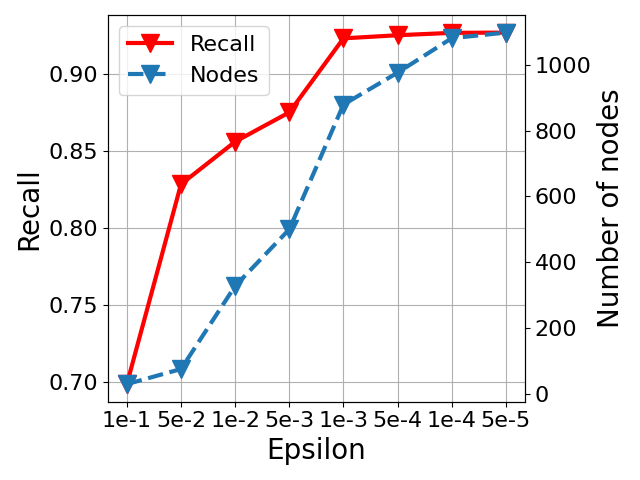
\includegraphics[width=0.65\linewidth,height=3.7cm]{figures/epsilon_metrics.png}
    \vskip -0.1in
    \caption{The relationship among Epsilon, Recall, and Node number. Note that the recall has reached 70\% with $\epsilon = 10^{-1}$ merely, and the increment of recall becomes slow when $\epsilon$ is less than $10^{-3}$.}
    \label{fig:epsilon_metrics}
\end{figure}
The approximation parameter $\epsilon$ is an important hyper-parameters in modulating the scalability.
To examine the effect of $\epsilon$ on the performance, we repeat experiments with different values of $\epsilon$ and report the recall as well as the number of traced nodes. 
As Figure \ref{fig:epsilon_metrics} shows, the recall has reached 70\% when $\epsilon = 10^{-1}$.
When $\epsilon$ is less than $10^{-3}$, the increment of recall becomes slow, and the number of nodes rapidly increases. 
Therefore, setting $\epsilon = 10^{-3}$ can guarantee a higher recall and fewer nodes with a relatively low cost in experiments, and we set $\epsilon = 10^{-3}$ for TRacer.
% , which is the reason why we set $\epsilon = 10^{-3}$ for TRacer.


% 对比实验
\subsubsection{Comparative experiment}
\begin{table}[t]
  \caption{
  Performance comparison between baselines and TRacer
%   Comparative experiment results. Besides the number of tracing nodes being more than APPR slightly, the recall and tracing depth are better than other methods significantly.
  }
  \label{tab:compared_methods}
  \begin{tabular}{cccc}
    \toprule
    Methods & Recall (\%) & Number of nodes (K) & Tracing depth\\
    \midrule
    BFS & 77.02 & 52.50 & 2.00\\
    Poison & 70.06 & 41.45 & 2.00\\
    Haircut & 58.85 & 10.35 & 4.15\\
    APPR & 71.92 & \textbf{0.66} & 3.60\\
    \textbf{TRacer} & \textbf{92.31} & 0.87 & \textbf{5.05}\\
  \bottomrule
\end{tabular}
\end{table}
Table \ref{tab:compared_methods} shows the performance of different methods, from which we can obtain the following observations.
\textbf{\textit{Firstly}}, the output graphs of BFS and Poison contain an extremely large number of nodes, which brings great difficulty to transaction auditing even through detecting more than 70\% target nodes.
\textbf{\textit{Secondly}}, the output graph of Haircut has fewer nodes than BFS and Poison with a greater tracing depth, but the recall is too low to achieve effective tracing.
\textbf{\textit{Thirdly}}, fewest nodes are obtained by APPR, ensuring the detection results can be easier audited by experts. 
\textbf{Fourthly}, TRacer obtains better performance than APPR. On the basis of the advantages of APPR, the recall and tracing depth of TRacer are significantly better than other methods.

% 消融实验
\subsubsection{Ablation experiment}
\begin{table}[t]
  \caption{Ablation experiment.}
  \label{tab:ablation_experiment}
  \setlength{\tabcolsep}{0.1mm}{
  \begin{tabular}{p{2.5cm}<{\centering}p{1.4cm}<{\centering}p{2.2cm}<{\centering}|p{0.6cm}<{\centering}p{1.8cm}<{\centering}}
    \toprule
    Graph construction with DeFi patterns & Graph expansion & Local community detection & Recall (\%) & Number of nodes (K)\\
    % pattern recognition & expansion & detection & (\%) & of nodes (K)\\
    \midrule
    $\surd$ & $\surd$ & $\surd$ & 92.3 & 0.87\\
     & $\surd$ & $\surd$ & 80.3 & 0.55\\
    $\surd$ & $\surd$ &  & 95.9 & 57.5\\
  \bottomrule
\end{tabular}}
\end{table}
TRacer is consist of three modules including graph construction, graph expansion, and local community detection. 
In order to discuss the function of different modules, we conduct an ablation study and report the performance of TRacer in Table \ref{tab:ablation_experiment} after removing the DeFi pattern recognition in graph construction and the local community detection.
% remove the graph construction module recognizing the edge patterns or local community detection module extracting the important local community, and report the performance as shown in Table \ref{tab:ablation_experiment}.
When the DeFi pattern recognition is removed in the graph construction module, the recall decreases significantly, which shows that the understanding of DeFi patterns in TRacer can help trace the money flows effectively.
Moreover, if the local community detection module is removed, the number of nodes increases significantly with the weakly improvement of recall, which shows that the local community detection module can find the nodes strongly associated with the source node at the cost of a small recall loss.

% Top N recall
\subsubsection{Top\textit{N} Recall}
\begin{figure}[t]
    \centering
    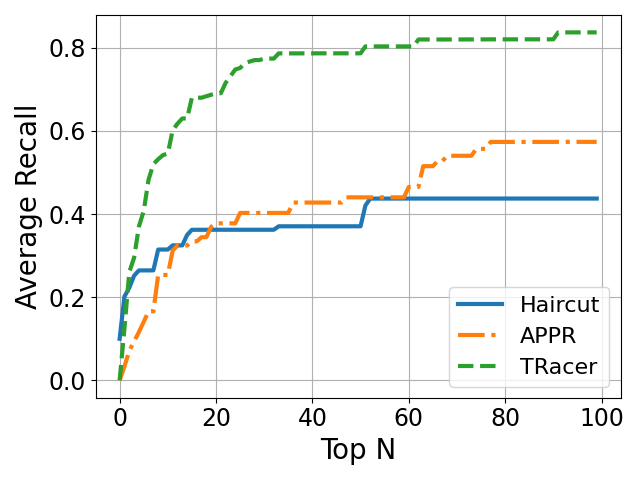
\includegraphics[width=0.6\linewidth]{figures/topn_recall_v2.png}
    \caption{Top $n$ most relevant nodes and the recall. 
    % TRacer tends to give higher importance to the target nodes.
    }
    \label{fig:topn_recall}
\end{figure}

Since the rank of a node represents the relevance relationship between this node and the source node, we can audit the nodes according to the descending order of rank. To compare the rank-based methods including Haircut, APPR, and TRacer, we take out the top $n$ most relevant nodes to the source and calculate the recall for different $n$.
The result is displayed in Figure \ref{fig:topn_recall}, where the curve of TRacer shows a better performance than other methods.
In addition, TRacer achieves a 25\% recall gain over APPR when $n>50$.

\subsection{Case Study}
\label{sec:case_study}
% 该部分对案例中的TTR局部交易网络进行分析
% In this part, we visualize the fund flow on cases with verified labels by Gephi 0.9.2 \cite{bastian2009gephi}.
In this part, we visualize the traced money flow of two cases with Gephi 0.9.2 \cite{bastian2009gephi}, in order to evaluate the feasibility of TRacer.
% In this section, we give the analysis of cases with the local tracing network captured by our method through gephi.

\subsubsection{Cryptopia}\label{sec:case_study_Cryptopia}
\begin{figure}[t]
    \centering
    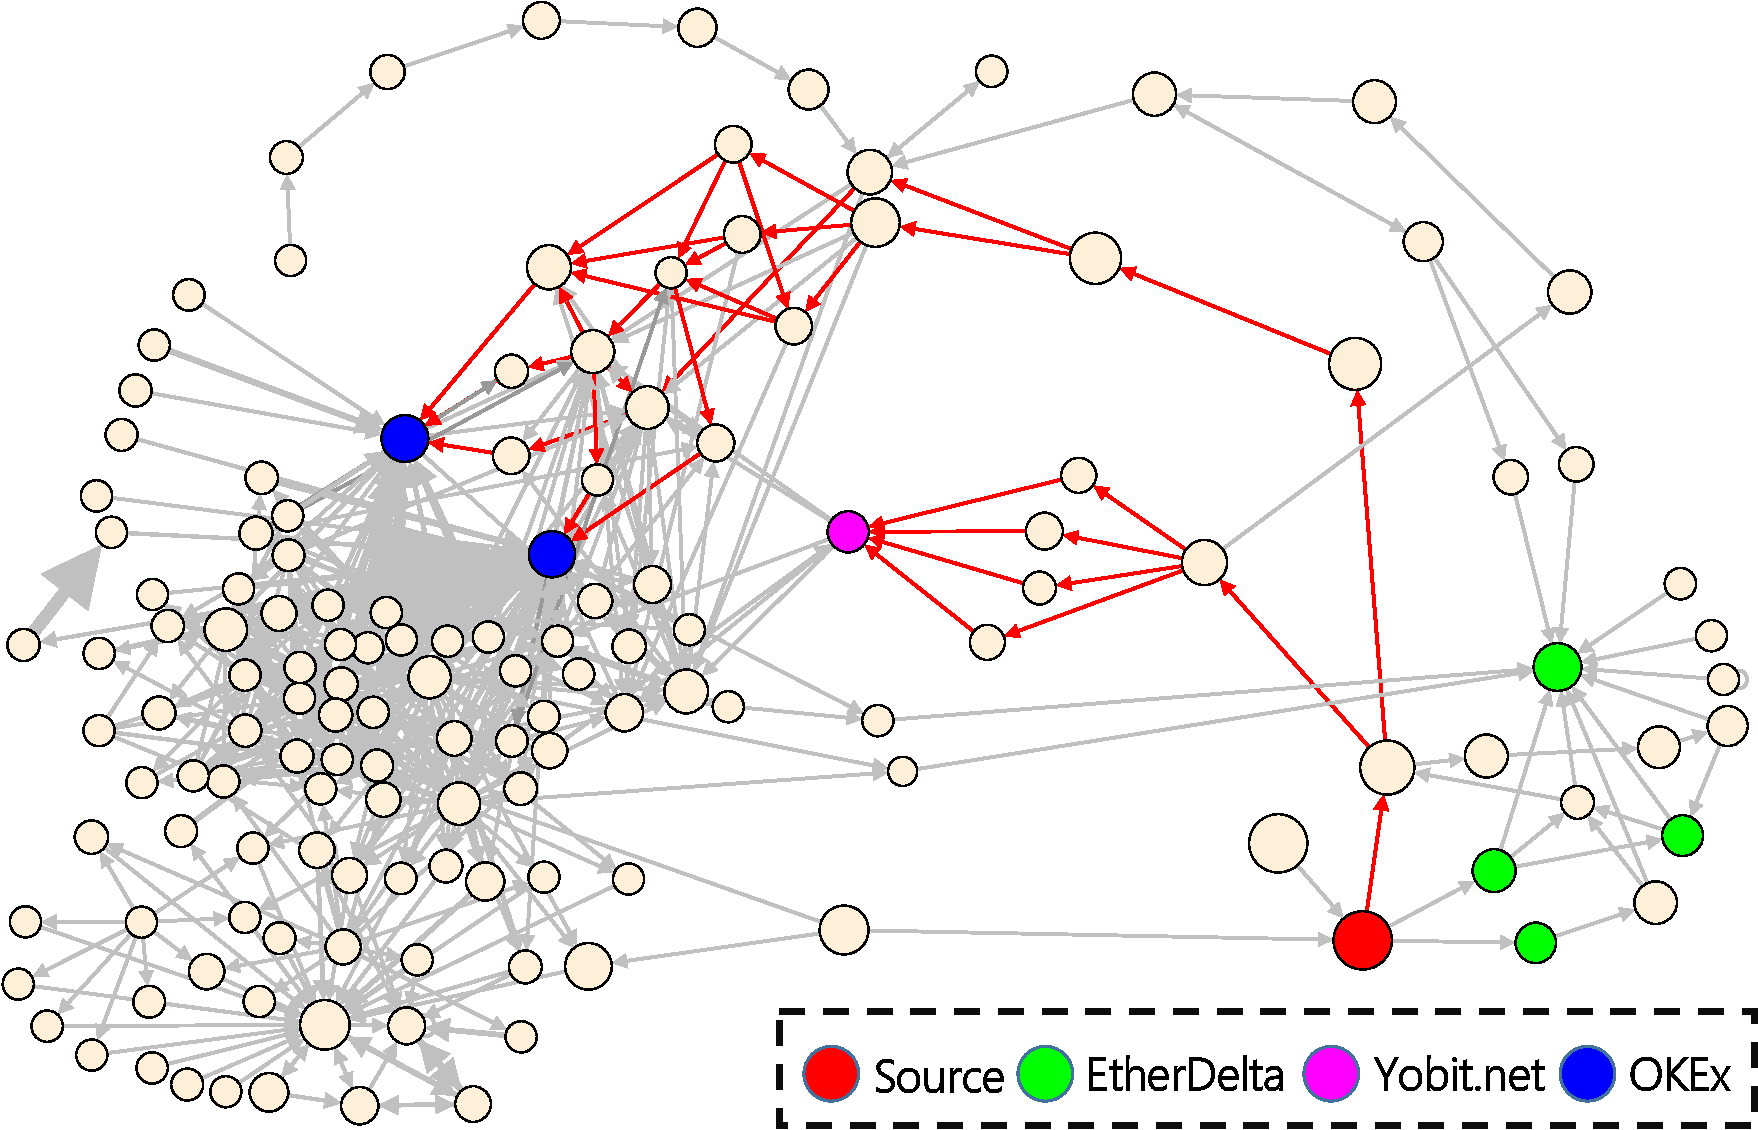
\includegraphics[width=0.8\linewidth]{figures/cryptopia.pdf}
    \caption{Tracing visualization for Cryptopia. Besides the EtherDelta exchange marked by experts, our method also finds the other target exchanges including Yobit.net and OKEx.}
    \label{fig:ttr_example_cryptopia}
\end{figure}
The Cryptopia exchange was attacked by hackers in May 2019.
According to the tracing result published by CoinHolmes\footnote{https://trace.coinholmes.com}, the source node with prefix 0xd4e79 \footnote{https://etherscan.io/address/0xd4e79226f1e5a7a28abb58f4704e53cd364e8d11} possessed 30.8K stolen ETH from Cryptopia and transferred about 10K ETH to 4 target nodes labeled as EtherDelta.

Figure \ref{fig:ttr_example_cryptopia} presents the transaction tracing result of our method, where the source node and the target nodes are marked with labels. 
Additionally, the node size is proportional to its rank score for each node, so the higher the rank is, the larger the node diameter is.
Based on the tracing result, we can find 4 target nodes labeled as EtherDelta (an exchange) in the 2-hop neighborhood of the source node easily, which is consistent with the results in CoinHolmes.

Moreover, another 4-hop neighbor of the source node labeled as Yobit.net\footnote{https://etherscan.io/address/0xf5bec430576ff1b82e44ddb5a1c93f6f9d0884f3} and two nodes labeled as OKEx can be found in the figure, which is not reported by CoinHolmes.
In fact, Yobit.net and OKEx are exchanges enabling the hacker to cash out the stolen ETH.
% In this way, Yobit.net and OKEx are reasonable to be target nodes.
According to the traced money flows in the figure, about 1420 stolen ETH is transferred into Yobit.net, and 18.47K stolen ETH is transferred into OKEx.
Therefore, more than 97\% of the stolen ETH of Cryptopia are traced by our method in this case. 

% Moreover, another 4-hop neighbor of the source node, labeled as Yobit.net with the address prefix 0xf5bec \footnote{https://etherscan.io/address/0xf5bec430576ff1b82e44ddb5a1c93f6f9d0884f3}, can also be found in the figure, which is not discovered by CoinHolmes.
% In fact, Yobit.net is an exchange enabling the hacker to cash out the stolen ETH, which is reasonable to be a target node.
% And from these fund flow paths, we can find the other 1420 stolen ETH.

% Besides, we can find two nodes labeled as OKEx in the figure, which is the deposit address of the OKEx exchange. 
% According to the traced ETH flows in the figure, it's reasonable that the hackers cashed out another part of the stolen ETH via OKEx, which is about 18.47K ETH.
% Therefore, more than 97\% of the stolen ETH of Cryptopia can be found with our method in this case.

\subsubsection{Kucoin}
\begin{figure}[t]
    \centering
    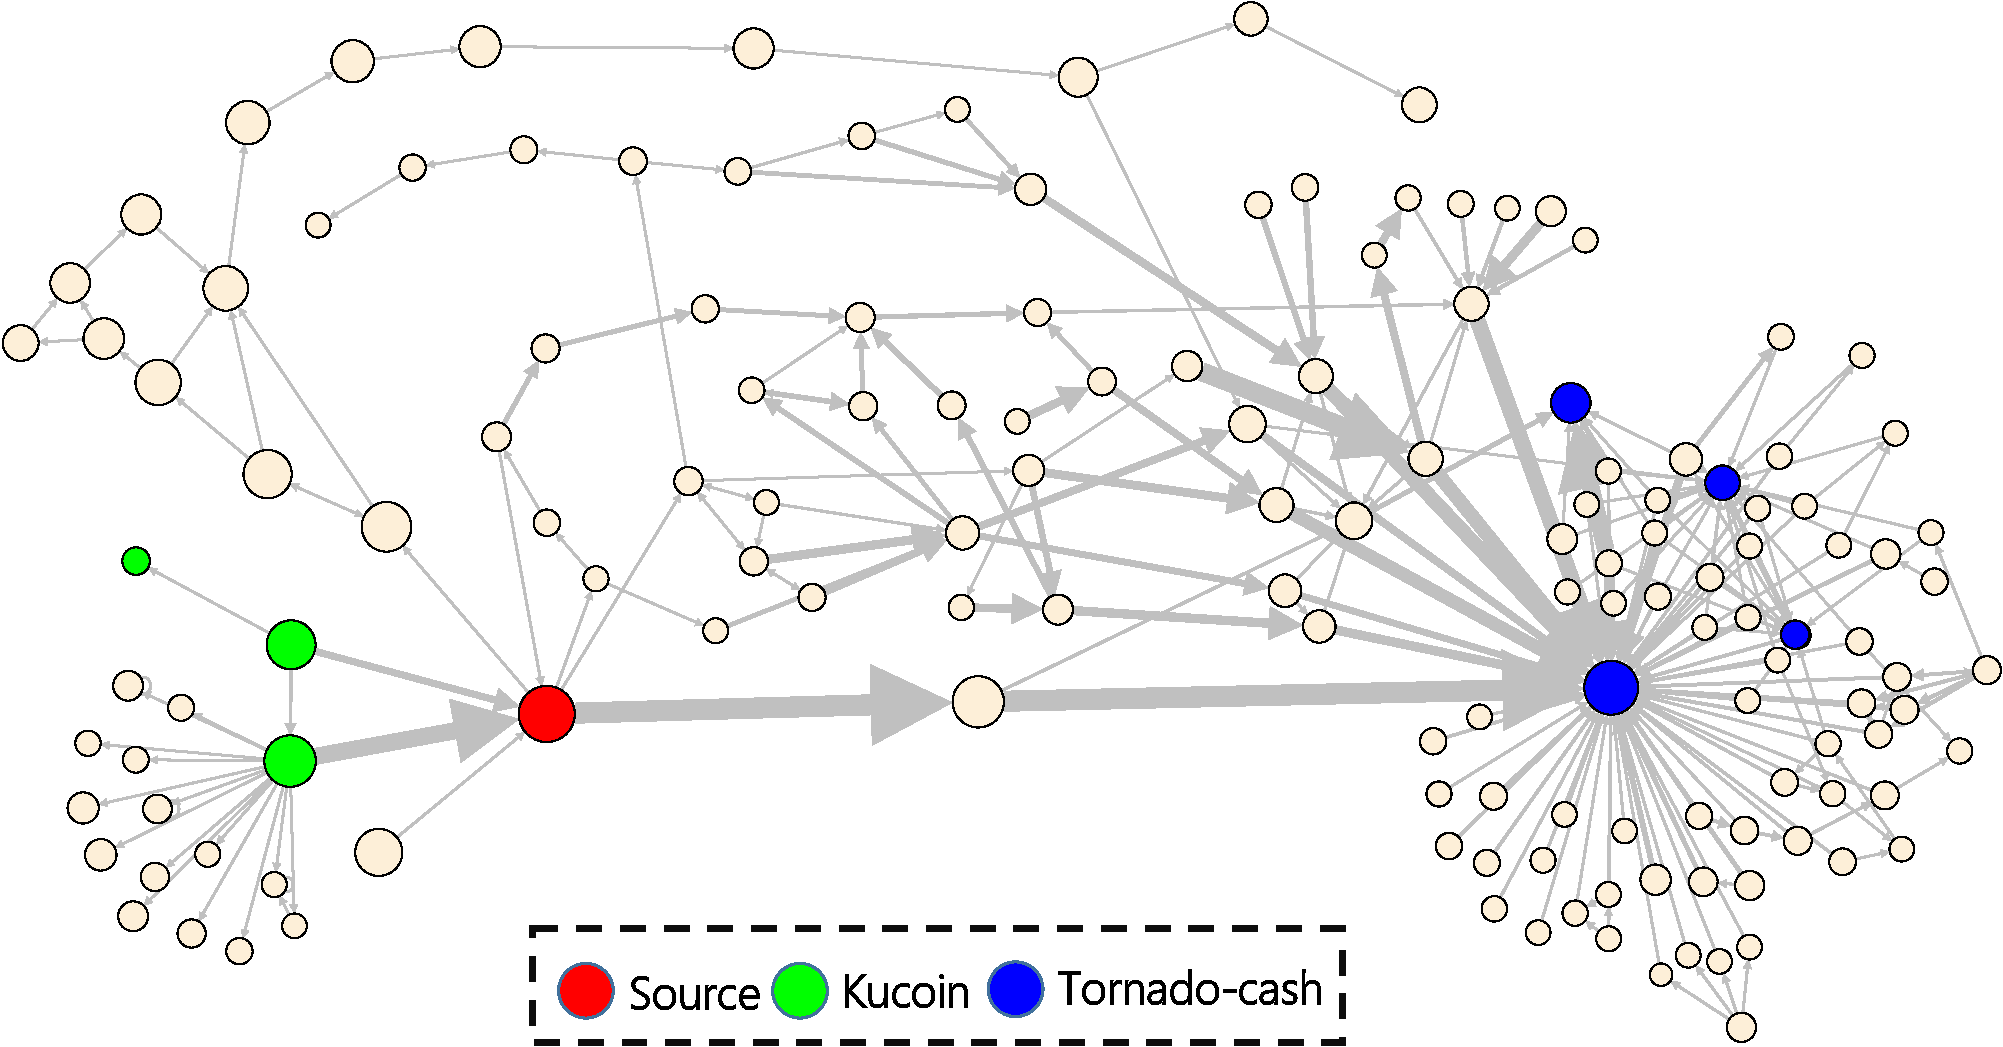
\includegraphics[width=0.95\linewidth]{figures/kucoin.pdf}
    \caption{Tracing visualization for Kucoin. A large number of ETH was transferred to Tornado Cash.}
    \label{fig:ttr_example_kucoin}
\end{figure}
The Kucoin exchange was attacked by hackers in September 2020, and there is still a large number of stolen funds that have not been traced until now.
As shown in Figure \ref{fig:ttr_example_kucoin}, the source node \footnote{https://etherscan.io/address/0xeb31973e0febf3e3d7058234a5ebbae1ab4b8c23} of the hackers obtained ETH from the nodes labeled as Kucoin, and then transferred most of the stolen ETH to a famous privacy-preserving protocol named Tornado Cash \cite{tornadocashdoc}.

Through the tracing result of our method, a total amount of 13.8K ETH was transferred to the 100 ETH pool of Tornado Cash, which is similar to the conclusion of experts in SlowMist\footnote{https://coinyuppie.com/uncovering-tornado-cashs-anonymity/}. As Tornado Cash is a decentralized mixing service, it is impossible for us to obtain valuable KYC information from this project to identify the hackers. 
In addition, since Tornado Cash is designed based on zero-knowledge proof, liquidity mining, and smart contract, it is difficult to trace the downstream fund flow when money is transferred into Tornado Cash. Therefore, some researchers have conducted analysis on Tornado Cash in recent years \cite{beres2020blockchain}.